% ---------------------------------------------------------------------------
% AXI4-Stream: un unico canal de datos unidireccional, sin canales de
% direccion ni de respuesta. El flujo lo validan TVALID/TREADY y lo cierra
% TLAST.
%
% Compilar:  pdflatex diagrama_axi_stream.tex
% ---------------------------------------------------------------------------
\documentclass[border=8pt]{standalone}
\usepackage[utf8]{inputenc}
\usepackage[T1]{fontenc}
\usepackage{lmodern}
\usepackage{tikz}
\usetikzlibrary{arrows.meta, calc, positioning}

\definecolor{cPropio}{HTML}{2A78D6}   % azul: logica de diseno propio
\definecolor{cIP}{HTML}{EDA100}       % ambar: IP de terceros
\definecolor{cExt}{HTML}{1BAF7A}      % aguamarina: software y hardware externo
\definecolor{cRef}{HTML}{8A8A85}      % gris: lineas y contornos

\tikzset{
    box/.style={draw, line width=0.9pt, rounded corners=2pt, align=center,
                font=\sffamily\small, inner sep=3pt},
    blk/.style={box, draw=cPropio, fill=cPropio!7},
    chanS/.style={-{Stealth[length=6pt]}, line width=1.7pt, cPropio!55!black},
    tok/.style={draw=cRef!65, fill=cRef!12, rounded corners=1.5pt,
                minimum height=0.5cm, minimum width=1.0cm,
                font=\ttfamily\scriptsize, inner sep=1pt},
    last/.style={tok, draw=cIP!85!black, line width=1.1pt, fill=cIP!16},
    chname/.style={font=\sffamily\scriptsize, text=cRef!22!black, inner sep=1pt},
    note/.style={font=\sffamily\scriptsize, text=cRef!45!black, inner sep=1pt},
    sig/.style={-{Stealth[length=4pt]}, line width=0.7pt, cRef!80!black},
}

\begin{document}
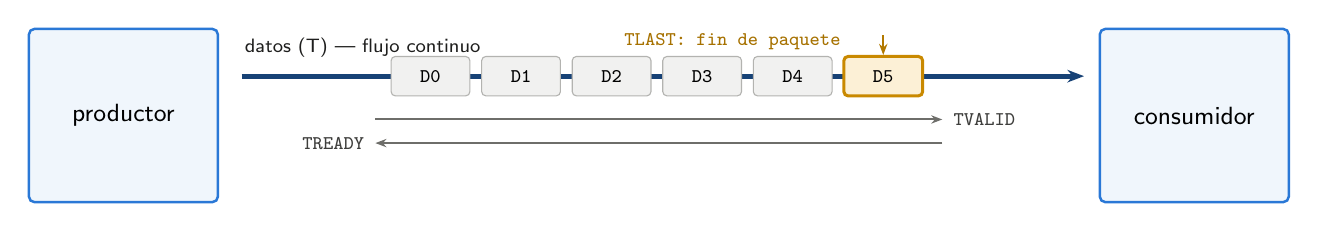
\begin{tikzpicture}[x=1cm, y=1cm, font=\sffamily\small]

\node[blk, minimum width=2.4cm, minimum height=2.2cm] at (1.2,1.9) {productor};
\node[blk, minimum width=2.4cm, minimum height=2.2cm] at (14.8,1.9) {consumidor};

% unico canal: datos (T), del productor al consumidor
\draw[chanS] (2.7,2.4) -- (13.4,2.4);
\node[chname, anchor=west] at (2.7,2.76) {datos (T) \textemdash{} flujo continuo};
\foreach \i in {0,1,2,3,4}{\node[tok] at ({5.1+\i*1.15},2.4) {D\i};}
\node[last] (tl) at ({5.1+5*1.15},2.4) {D5};
\draw[sig, cIP!75!black] ({5.1+5*1.15},2.92) -- (tl.north);
\node[note, text=cIP!70!black, anchor=east] at ({5.1+5*1.15-0.5},2.84)
     {\ttfamily TLAST: fin de paquete};

% handshake: TVALID/TREADY validan cada palabra
\draw[sig] (4.4,1.85) -- (11.6,1.85);
\node[note, anchor=west] at (11.7,1.85) {\ttfamily TVALID};
\draw[sig] (11.6,1.55) -- (4.4,1.55);
\node[note, anchor=east] at (4.3,1.55) {\ttfamily TREADY};

\end{tikzpicture}
\end{document}
